\documentclass[border=10pt]{standalone}
\usepackage{tikz}
\usetikzlibrary{calc}

\definecolor{layer0}{HTML}{1F6FB2}
\definecolor{layer1}{HTML}{2E9E44}
\definecolor{layer2}{HTML}{C8372D}
\definecolor{link}{HTML}{555555}
\definecolor{grid}{HTML}{B0B0B0}

\newcommand{\points}{%
  0/-1/-1/1, 1/0/-1/1, 2/1/-1/1,
  3/-1/-1/0, 4/0/-1/0, 5/1/-1/0,
  6/-1/-1/-1, 7/0/-1/-1, 8/1/-1/-1,
  9/-1/0/1, 10/-1/0/0, 11/-1/0/-1,
  12/1/0/-1, 13/1/0/0, 14/1/0/1,
  15/-1/1/-1, 16/0/1/-1, 17/1/1/-1,
  18/-1/1/0, 19/0/1/0, 20/1/1/0,
  21/-1/1/1, 22/0/1/1, 23/1/1/1}

\tikzset{
  board/.style={line width=2pt, line cap=round},
  cubegrid/.style={grid, dashed, line width=0.6pt},
  point/.style={circle, draw, line width=1.4pt, fill=white, minimum size=7mm, inner sep=0pt, font=\sffamily\bfseries\small},
  centre/.style={circle, draw=grid, dashed, line width=0.8pt, fill=white, minimum size=3mm, inner sep=0pt}
}

\begin{document}

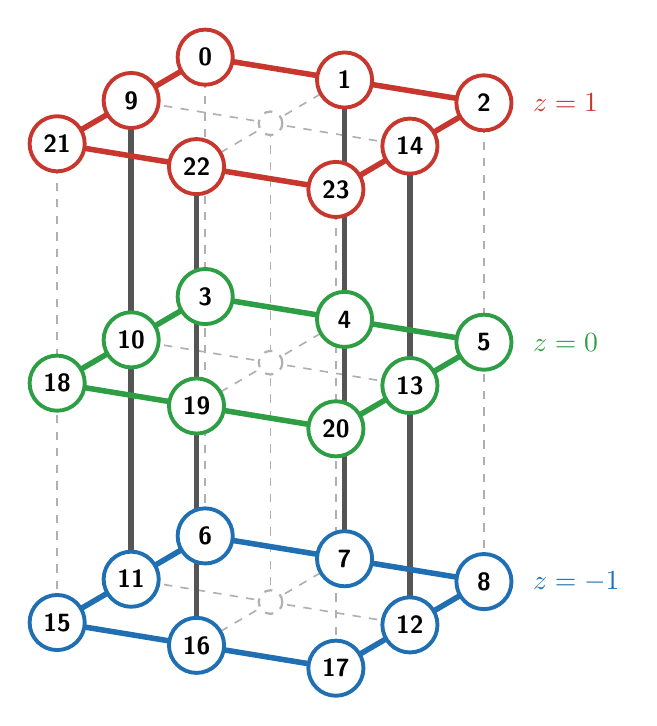
\begin{tikzpicture}[x={(1.77cm,-0.29cm)}, y={(-0.94cm,-0.55cm)}, z={(0cm,3.04cm)}]
  \foreach \z in {-1, 0, 1} {
    \foreach \x/\y in {1/0, -1/0, 0/1, 0/-1}
      \draw[cubegrid] (0, 0, \z) -- (\x, \y, \z);
  }
  \foreach \x/\y in {-1/-1, 1/-1, 1/1, -1/1, 0/0}
    \draw[cubegrid] (\x, \y, -1) -- (\x, \y, 1);
  \foreach \x/\y in {0/-1, 1/0, 0/1, -1/0}
    \draw[board, link] (\x, \y, -1) -- (\x, \y, 1);
  \foreach \z in {-1, 0, 1} {
    \pgfmathtruncatemacro{\c}{\z + 1}
    \draw[board, layer\c] (-1, -1, \z) -- (1, -1, \z) -- (1, 1, \z) -- (-1, 1, \z) -- cycle;
    \node[centre] at (0, 0, \z) {};
    \node[font=\sffamily\bfseries, text=layer\c, anchor=west] at ($(1, -1, \z) + (0.5cm, 0)$) {$z = \z$};
  }
  \foreach \n/\x/\y/\z in \points {
    \pgfmathtruncatemacro{\c}{\z + 1}
    \node[point, draw=layer\c] at (\x, \y, \z) {\n};
  }
\end{tikzpicture}

\end{document}
